\chapter{Unity and Developing for HoloLens}\label{sec:unity}
%\chapterprecis{Our hero is introduced; family tree; early days.}
Unity is a cross-platform game engine developed by Unity Technologies. It has been widely known for its ease of use and easy portability to different platforms. Even though Unity's primary focus is the creation of 2D and 3D games, it has also been known to be versatile in the creation of other realtime applications. In cooperation with Microsoft, Unity now includes support for HoloLens, Microsoft's latest mixed-reality device.\par

HoloLens Apps can be created in a variety of ways which include implementing them as Universal Windows Apps, DirectX projects or Unity Applications. Unity was chosen for this Project because of it's ease of use and intuitive workflow.

\section{Unity Overview}
A Unity Project contains four main elements: Assets, Scenes, GameObjects and Components. These elements interact with each other in different ways to create the final application.

\subsection{Assets}
Assets are the main content of any Unity Project. These can include 3D-models, textures, audio files software-libraries etc. Usually, most of the Assets are created using external software and then imported into the project.

\subsection{Scenes}
A Scene is a self-contained 3D space where all interaction happens. Every Unity Project needs to have at least one Scene. Scenes are the 3D space where Assets can exist. Most projects will have multiple Scenes. The most common use of Scenes in game development is to create different levels inside a game, however this will largely depend on the project specifications and design. Although a Unity Project can may have as many Scenes as necessary, it is important to state that only one Scene is active and running at a given time. Unity manages Assets in a Scene in form of GameObjects.

\subsection{GameObjects}
A GameObject is Unity's base entity. For an Asset to exist in a Scene, it has to be a GameObject. A GameObject by itself does not have any sort of behavior, other than that it exists inside a Scene. To give GameObjects meaningful behavior, so called Components have to be attached to a GameObject.

\subsection{Components}
A Component is responsible for assigning roles, properties and/or behaviors to GameObjects. Unity provides a wide variety of components such as lighting, colliders and physics bodies etc. which can be used to change the behavior of GameObjects. Custom behavior through scripting is also added to GameObjects through Components.



\section{Working with Unity}
Unity's primary focus is that of an game-engine, thus most Assets will be created in separate applications. The typical Unity workflow includes creating Assets, importing and configuring them inside Unity and adding logic through scripting.

\subsection{Unity Editor}
Unity manages its user interface through different windows. The default user interface contains the most used windows, which include:

\subsubsection{Project Window}
This view acts as a file browser where all Assets that belong to the project can be viewed. Assets can be organized by grouping them in folders. The project window also has search function to quickly find certain Assets.
\begin{figure}[H]
  \centering
  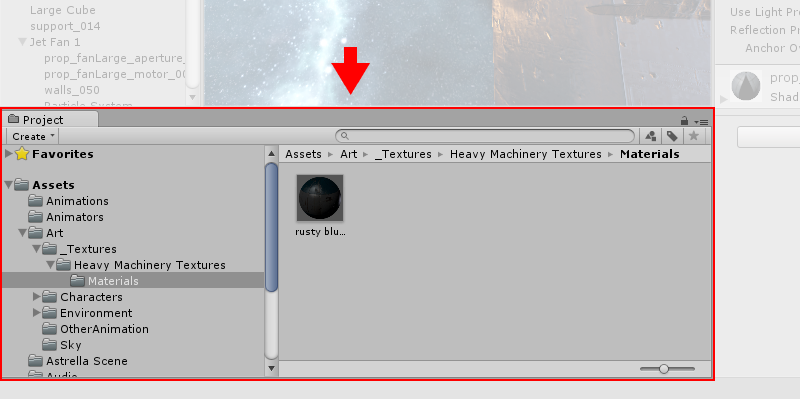
\includegraphics[width=0.4\textwidth]{images/ProjectWindow.png}
  \caption{Project Window}
\end{figure}

\subsubsection{Scene View}
The Scene View is the interactive view into the world that is created. The Scene View is used to select and position scenery, objects, cameras, lights, and all other types of Game Objects. 
\begin{figure}[H]
  \centering
  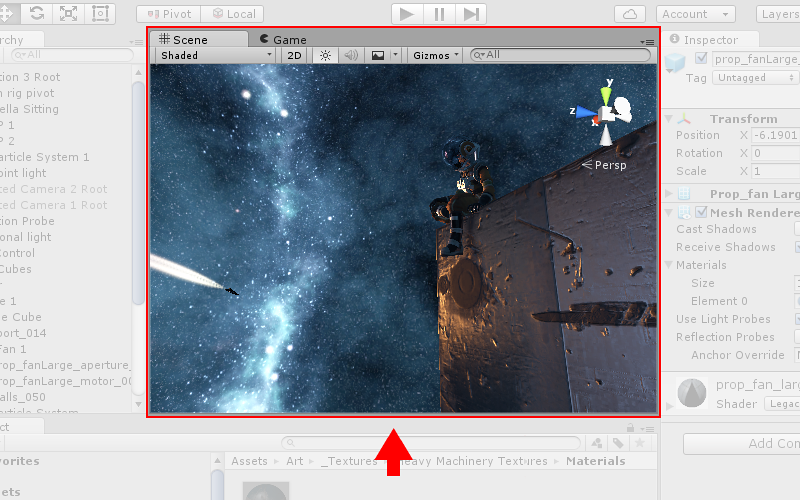
\includegraphics[width=0.4\textwidth]{images/SceneView.png}
  \caption{Scene View}
\end{figure}

\subsubsection{Game view}
The Game View is rendered from the Camera(s) in the Scene. It is representative of the final, published application. One or more cameras are needed to control what the user actually sees when they are using the application.
\begin{figure}[H]
  \centering
  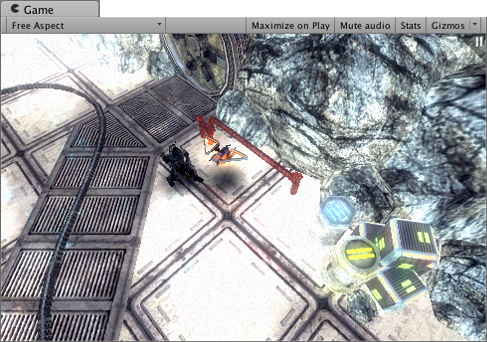
\includegraphics[width=0.4\textwidth]{images/GameView.png}
  \caption{Game View}
\end{figure}

\subsubsection{Hierarchy window}
The Hierarchy window contains a list of every Game Object in the current Scene. Some of these are direct instances of Asset files (like 3D models), and others are instances of Prefabs, which are custom objects that make up most of your game. As objects are added and removed in the Scene, they will appear and disappear from the Hierarchy as well. By default, objects are listed in the Hierarchy window in the order they are made. Objects can be re-ordered by dragging them up or down, or by making them “child” or “parent” objects.
\begin{figure}[H]
  \centering
  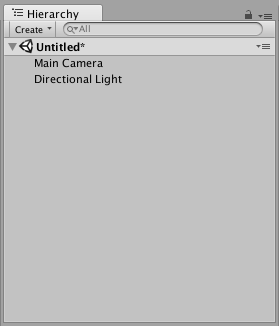
\includegraphics[width=0.2\textwidth]{images/Hierarchy.png}
  \caption{Hierarchy Window}
\end{figure}

\subsubsection{Inspector window}
The Inspector is used to view and edit the properties and settings of Game Objects, Assets, and other preferences and settings in the Editor. When a GameObject is selected in the Hierarchy or Scene View, the Inspector will show the Properties of all Components and Materials on that object which can be edited. The image below shows the inspector with the default 3D camera GameObject selected. In addition to the object’s position, rotation and scale values, all the properties of the camera are available to edit.
\begin{figure}[H]
  \centering
  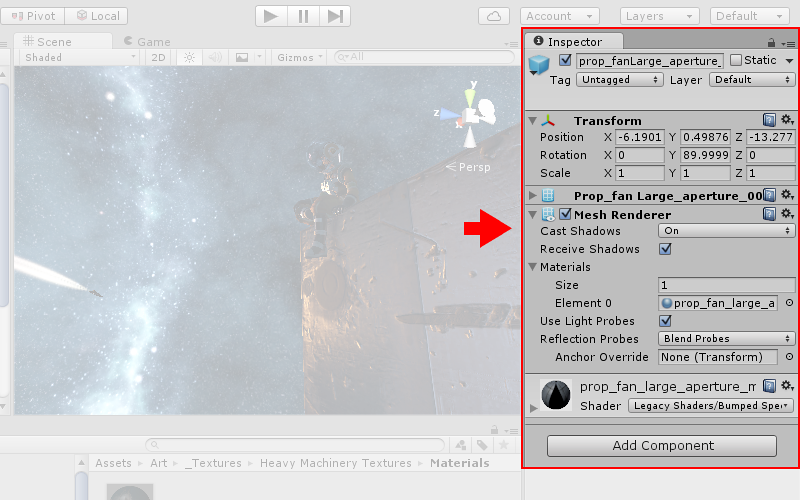
\includegraphics[width=0.4\textwidth]{images/InspectorWindow.png}
  \caption{Inspector Window}
\end{figure}
A more in-depth overview of how to use Unity can be found in the official Unity manual\footnote[1]{https://docs.unity3d.com/Manual/UnityOverview.html, last visited 27th February 2017}

\section{Asset Workflow}
When creating applications in Unity, the typical workflow involves importing Assets, configuring certain settings, adding components to GameObjects and adding custom behavior to those GameObjects through scripting.

\subsection{Importing/Adding Assets}
Unity supports a wide variety of file types to be used as Assets, some common file types include:
\begin{itemize}
\item Image files
\item 3D Model files
\item Meshes \& Animations
\item Audio files
\end{itemize}
Each file type has it's own import settings, which show up in the inspector when a file is imported, and can be configured to suit the specific needs like quality, compression etc. Assets can also be imported from Asset-Packages, exported from other projects or from the Unity Asset Store. Being primarily a 3D game engine, Unity can work with 3D models of any shape that can be created with modeling software. However, there are also a number of primitive object types that can be created directly within Unity, which include 
\begin{itemize}
\item Cube
\item Sphere
\item Plane
\item Capsule
\end{itemize}
These objects can be added through the \textbf{GameObject \textgreater 3D Object \textgreater Cube/\newline/Sphere/Plane/Capsule} panel. These basic primitives can act as placeholder objects which can be replaced for more complex 3D models later on.

\subsection{Scripting}
Unity provides its own API to manipulate GameObjects. This is known as Scripting. Scripts are code files which can be added to GameObjects as Components to achieve the desired behavior. Scripting can be done in two languages: C\# or UnityScript (usually called JavaScript). UnityScript is Unity's own scripting language with a syntax similar to JavaScript, yet the two languages are not the same. Usage of C\# in Unity is basically as one would expect. Even though both languages can be used in the same project, it is not recommended to do so for obvious reasons. Generally, C\# is considered to be the better choice for scripting.

\subsubsection{Creating and Using Scripts}
Scripts are usually created within Unity directly. A new script can be created from the Create menu at the top left of the Project panel or by selecting \textbf{Assets \textgreater\xspace Create \textgreater\xspace C\# Script (or JavaScript)} from the main menu. The new script will be created in whichever folder is selected in the Project panel. The new script file’s name will be selected, prompting to enter a new name.
\begin{figure}[H]
  \centering
  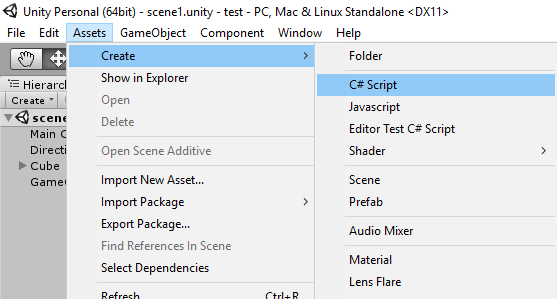
\includegraphics[width=0.4\textwidth]{images/CreateScript.png}
  \caption{Creating a Script}
\end{figure}
\begin{figure}[H]
  \centering
  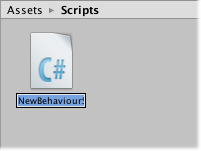
\includegraphics[width=0.2\textwidth]{images/NewScriptIcon.png}
  \caption{Script as it appears in the Project Window after creation}
\end{figure}
\subsubsection{Editing Scripts}
By default, the initial contents of a newly added Script will be the following:
\begin{lstlisting}
using UnityEngine;
using System.Collections;

public class CustomScript : MonoBehaviour {

    // Use this for initialization
    void Start () {
    
    }
    
    // Update is called once per frame
    void Update () {
    
    }
}
\end{lstlisting}
Unity's default editor for Scripts is MonoDevelop, though this can be changed to Visual Studio or any other editor of choice under the External Tools panel in the Preferences menu.

\subsubsection{MonoBehaviour}
A script makes its connection with the internal workings of Unity by implementing a class which derives from the built-in class \textbf{MonoBehavior}. Creating a new Script is basically creating a new Component-type that can be attached to a GameObject. Each time a Script Component is attached to a GameObject, it creates a new instance of the object defined by the Script. The name of the class is taken from the name supplied when the file was created. The class name and file name must be the same to enable the script component to be attached to a GameObject. Scripts can be added to GameObjects either by dragging them onto GameObjects via the Unity Editor or In-Code by using the \textit{AddComponent \textless \textgreater}()-function derived from MonoBehavior:
\begin{lstlisting}
void Start () {
	
    this.gameObject.AddComponent<ComponentToAdd>();
}
\end{lstlisting}
In Unity scripting, there are a number of event functions that get executed in a predetermined order over the lifecycle of the script. When creating a new script, the function bodies for \textit{Start()} and \textit{Update()} are generated automatically. To perform other actions, the corresponding MonoBehaviour functions can be overwritten. The following chart illustrates the available event functions:
\begin{figure}[H]
  \centering
  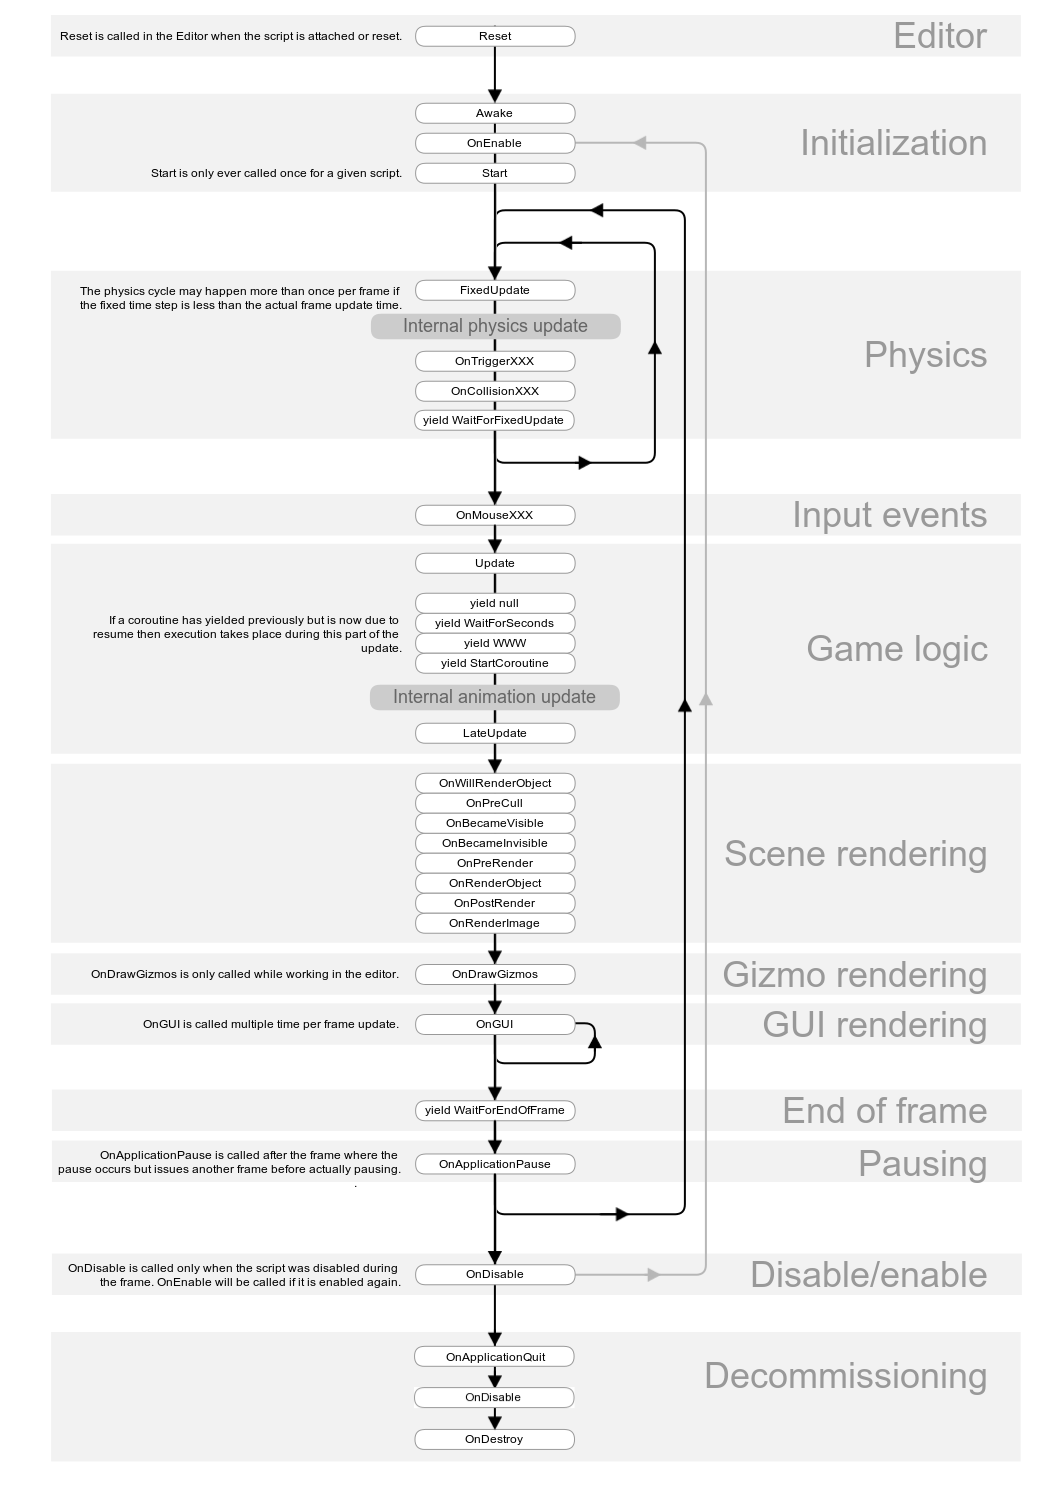
\includegraphics[width=1\textwidth]{images/MonoBehaviourFlowChart.png}
  \caption{MonoBehavior lifecycle}
\end{figure}

\newpage
\section{Deploying an App to HoloLens}
The build process of a Unity-based HoloLens-Apps differs from the build process of conventional Unity-Apps. Normally, a Unity Application can be run and debugged inside Unity itself, by using the toolbar:
\begin{figure}[H]
  \centering
  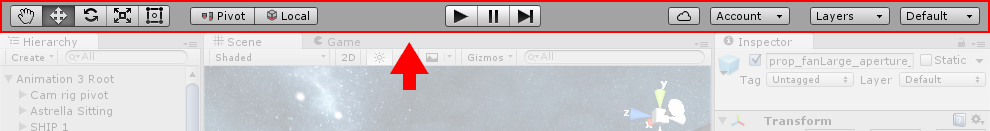
\includegraphics[width=0.8\textwidth]{images/Toolbar.png}
  \caption{Unity toolbar}
\end{figure} 
Conventional Unity applications can be run and debugged by pressing the \textit{Play}-button from the toolbar. HoloLens-applications require an extra step in order to be deployed to HoloLens, which involves generating a VisualStudio-Project which is then used to deploy to HoloLens. A detailed description on the standard deployment process can be found in the \textit{Holograms 100} tutorial\footnote[2]{https://developer.microsoft.com/de-DE/windows/holographic/holograms\_100, last visited 27th February 2017}

\subsection{Holographic emulation}
Holographic Emulation allows HoloLens applications to be run and debugged inside of Unity, which shortens deployment time significantly. During the development of this project, Holographic Emulation was still in beta and not available for usage. The current project runs with Unity 5.4, whereas Holographic Emulation is scheduled to be released with Unity 5.5.

\subsection{HoloToolkit}
The HoloToolkit is a collection of scripts and components intended to accelerate development of holographic applications targeting Windows Holographic. HoloToolkit version 1.5.4.0 was integrated into this project. During development, version 1.5.5.0 has been released, but not yet integrated into the project. HoloToolkit contains scripts supporting the following topics:
\begin{itemize}
\item Input
\item Sharing
\item Spatial Mapping
\item Spatial Sound
\item Utilities
\end{itemize}
HoloToolkit also provides an extension to the Unity user interface, featuring its own Build Window, allowing for a more streamlined deployment process.

\begin{figure}[H]
  \centering
  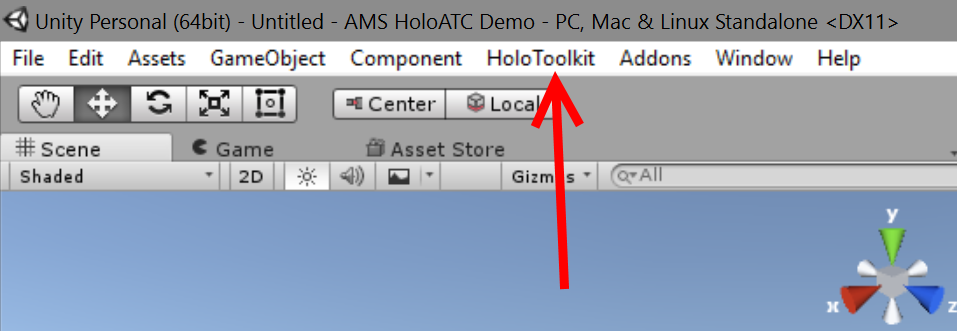
\includegraphics[width=0.8\textwidth]{images/HoloToolkitExtension.png}
  \caption{HoloToolkit extension}
\end{figure} 

\begin{figure}[H]
  \centering
  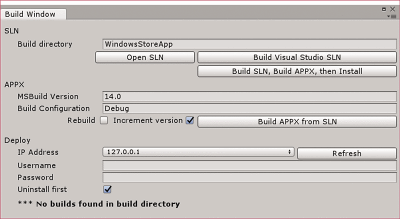
\includegraphics[width=0.8\textwidth]{images/HoloToolkitBuildWindow.png}
  \caption{HoloToolkit build window}
\end{figure} 







